\documentclass[12pt,a4paper,sans]{article}

\RequirePackage[utf8]{inputenc}
\usepackage[french]{babel}
\usepackage{amsmath} 
\usepackage{amsfonts} 
\usepackage{amssymb} 
\usepackage{graphicx} 
\usepackage[margin=0.8in]{geometry}
\usepackage{stackrel}
\usepackage{float}

\hyphenpenalty=10000
\frenchbsetup{StandardItemLabels=true}

\title{Simulation d'essaims particulaires}
\author{Keck Jean-Baptiste - Zirnhelt Gauthier}

\begin{document}

\maketitle



\section{Présentation du problème}

\subsection{Étapes de la simulation}
La simulation débute par l'initialisation d'un domaine de taille configurable avec des agents positionnés aléatoirement, aux propriétés également configurables.\\
La boucle de calcul pour la simulation de base est la suivante :
\begin{enumerate}
    \item Calcul des forces appliquées à chaque agent en fonction de tous ceux qui se trouvent à sa portée.
    \item Application des forces précédemment calculées à chaque agent.
    \item Sérialisation des données des agents dans un fichier.
\end{enumerate}
Si un agent sort du domaine pendant un pas de simulation, il est téléporté à l'opposé dans le domaine tout en gardant sa vitesse et sa direction.

\subsection{Coûts des étapes de la simulation}
L'évaluation des forces appliquées à chaque agent est l'opération la plus coûteuse de la simulation, car sa complexité est quadratiquement liée à celle du nombre d'agents à simuler. Les autres étapes n'ont en revanche qu'une complexité directement proportionnelle au nombre d'agents.\\
Nous avons donc dû privilégier l'accélération de l'étape de calcul des forces qui déjà dans le programme de base (640 agents) prenait plus de 99\% du temps de calcul total.



\newpage
\section{Solution implémentée}

\subsection{Dépendances}
% C++11 MANDATORY [insert perrier référence]
% building the solution = cmake + sm_20 pour cuda à cause de compil séparée
Notre base de code requiert :
\begin{itemize}
    \item un compilateur supportant le standard C++11
    \item une carte graphique Nvidia avec l'architecture $sm\_20$ au minimum (pour la compilation séparée des kernels CUDA)
    \item CMake 2.8.12 ou plus (CMake 3.x.x fortement conseillé à cause d'un bug connu dans la compilation des kernels CUDA)
    \item mpi? nvcc? thrust TODO 
    \item OpenGL 3.3 ou plus pour les programme effectuant un rendu 3D
\end{itemize}

Dans le cas où vous n'auriez pas un compilateur supportant C++11, nous fournissons un script qui permet de télécharger et installer GCC 4.8.2 sur votre machine (voir dans la sous-section Scripts utilitaires).\\\\

\subsection{Architecture générale}
% MPI / CUDA merged => mpirun -n 1 ou disable CUDA dans CMakeLists.txt
% les scripts (listés plus bas, pas détailler ici)
% différents éxecutables (sequential / tree???? / main(TODO rename it?) / display)
% différents tests (test_vec : vecteurs<T>           test_messenger : envoi/réception des messages MPI)
% les arbres utilisés
Nous avons opté pour un programme hybride permettant d'utiliser à la fois la performance du calcul distribué avec MPI et également celle du GPGPU avec CUDA. Il est toutefois toujours possible de tester notre programme avec seulement MPI ou seulement CUDA, respectivement en lançant un seul processus ou en désactivant CUDA dans les paramètres au début de $CMakeLists.txt$.\\\\

Les exécutables générés sont les suivants :
\begin{itemize}
    \item $sequential$ : Programme de simulation de base (sur CPU, un seul processus)
    \item $main$ : Programme de simulation hybride MPI / CUDA (TODO rename???)
    \item $display$ : Programme d'affichage des positions des agents simulés
    \item $tree$ : TODO
    \item $cuda tree$ : FAPFAPFAP TODO
    \item $barbecue$ : J'aime ta sauce Poulpy :D TODO
    \item $test\_vec$ : Programme de test des classes de vecteurs
    \item $test\_messenger$ : Programme de test de l'interface de communication construite sur MPI
\end{itemize}

Nous fournissons en outre gracieusement des scripts utilitaires pour paramétrer l'utilisation de MPI ou de préparer les données à la visualisation.

\subsection{MPI}
% Architecture centralisée seulement pour le load balancing
% Init par racine, puis scatter en fonction de la densité des agents et de leurs coordonnées.
% Chaque processus connait ses voisins et leur échange son agent moyen, ses agents "sortants". Il envoie aussi périodiquement sa charge d'agents à simuler au processus racine qui peut prendre la décision de rééquilibrer l'affectation des domaines aux processus.
% Réception des messages bloquante
% possibilité simu cpu bruteforce ou gpu

\subsection{CUDA}
% mémoire coalescente
% optimisations diverses...
% thrust

\subsection{Scripts utilitaires}
% Donner leur fonction
Les scripts utilitaires fournis avec nos sources sont les suivants :
\begin{itemize}
    \item $dependancies.sh$ : Installe les dépendances de GCC 4.8.2 
    \item $gcc.sh$          : Installe GCC 4.8.2 (pour le support de C++11)
    \item $genAppFile.sh$   : Génère un fichier Appfile automatiquement à partir d'une liste d'host en stdin.
    \item $merge\_files.py$ : Fusionne tous les fichiers de données issus de la simulation par des processus différents en un seul fichier.
    \item $path.sh$         : Corrige le $.bashrc$ des ensipc.
    \item $scanner.sh$      : Établit rapidement la liste des machines (ensipc) en ligne.
    \item $utils.sh$        : Contient des fonctions utilitaires utilisées par $gcc.sh$.
    \item $visu.sh$         : Script permettant de visualiser les résultats avec $gnuplot$ sur une machine ne permettant pas de compiler et/ou eexécuter le programme de visualisation d'agents fourni.
\end{itemize}

\subsection{Visualisation}
% Expliquer comment marche le viewer (merge fichiers, parsing fichier, sprites)
Nous fournissons un programme permettant de visualiser les agents simulés dans de meilleures conditions qu'avec gnuplot.
Celui-ci se lance avec la commande $./display$ et va par défaut lire le fichier résultant de l'opération de fusion réalisée par le script $merge\_files.py$. Il est possible de modifier le fichier lu par défaut en en spécifiant un autre à l'aide de l'option $-f$ du programme.\\

Le progamme affiche chaque agent sous la forme d'une sprite faisant face à la caméra. Cette sprite contient un cercle coloré représentant le type d'agent affiché. Cette technique de rendu très simple permet d'afficher beaucoup plus d'agents simultanément que si l'on représentait chaque agent par un volume texturé par exemple, ce qui permet de conserver une visualisation fluide pour grand nombre d'agents.\\

L'étape de la simulation en cours de visualisation est affichée en bas à gauche de l'écran. 
La lecture est pausable avec la touche $entr\acute{e}e$. 
Il est possible de rembobiner la simulation au démarrage en appuyant sur la touche $r$.
Les axes (utilisés pour avoir un repère fixe) sont affichables en utilisant la touche $a$.



\section{Résultats}
% En gros, surtout des images commentées

\begin{minipage}{0.33\textwidth}
	\begin{flushleft}
		\begin{figure}[H]
			\centering
			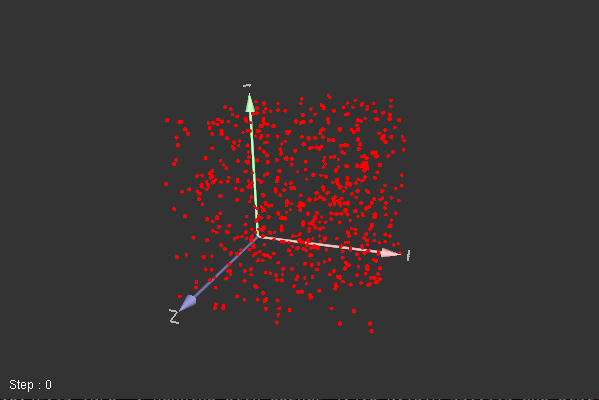
\includegraphics[width=\textwidth]{img/visu0.png}
			\caption{Début d'une simulation avec des agents aux positions, vitesses, et directions aléatoires}
		\end{figure}
	\end{flushleft}
\end{minipage}
\begin{minipage}{0.33\textwidth}
	\begin{flushright}
		\begin{figure}[H]
			\centering
			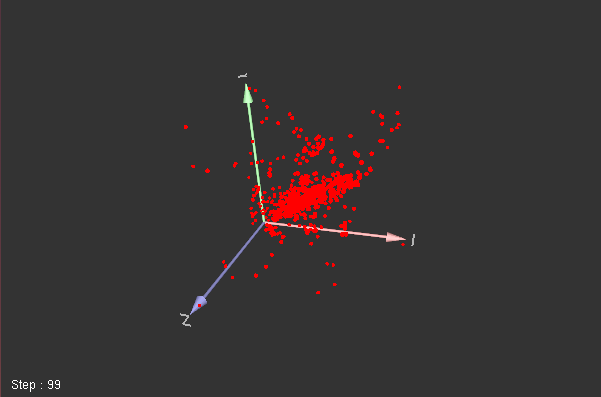
\includegraphics[width=\textwidth]{img/visu.png}
			\caption{Visualisation d'un essaim de particules formé durant la simulation}
		\end{figure}
	\end{flushright}
\end{minipage}\\



\section{Analyse des résultats}

\subsection{Performances}
% Tableau comparatif : méthode(sequential, mpi seul, cuda seul, hybride) / nombre de boids (100-1000-10k-1M-...) [/ nombre de process / gpu]
% Peut-être aussi en fonction des rayons?

\subsection{Qualité de la simulation}
% Vite dit, visuellement dans le viewer
% formation d'esseims avec la force de cohésion : ok
% force de séparation => esseims assez étalés : ok
% alignement dans un direction commune qui sera conservée sauf collisions : ok 
Nous avons fait des essais de simulation en modifiant les paramètres de la simulation et observé un comportement cohérent des agents lorsqu'une force était prépondérante sur les autres.
\begin{itemize}
    \item La force de cohésion permet la création d'essaims d'agents.
    \item La force de séparation sépare les agents afin de ne pas avoir d'essaims d'une densité trop élevée, mais peut aussi rendre impossible la formation de ces essaims si elle est trop grande.
    \item La force d'alignement force les agents à tous aller dans la même direction, ce qui permet globalement de conserver un essaim dans le temps tant qu'il n'entre pas en collision avec un autre.
\end{itemize}



\section{Perspectives d'amélioration}

\subsection{Tolérance à la faute pour MPI}
% timeout sur les messages MPI au lieu de bloquer indéfiniment.
Nous utilisons des messages MPI bloquants en réception, ce qui fait que notre système ne tolère aucune perte de message. Normalement, aucun message n'est perdu par MPI, mais dans le cas où une machine subit une défaillance, tout notre système se trouvera bloqué et il faudra recommencer la simulation.\\
Une amélioration consisterait ici à implanter un système tolérant à la faute en utilisant un système de timeout pour détecter les fautes, ainsi qu'un système de réplication des données des agents entre les différentes machines pour réaffecter les tâches de calcul.

\subsection{Visualisation de la simulation}
Nous aurions aimé avoir le temps nécessaire à l'amélioration de notre programme de visualisation. Les améliorations envisagées sont les suivantes :
\begin{itemize}
    \item Affichage à l'aide d'un triangle orienté de la direction d'un agent
    \item Sélection du numéro de l'étape à visualiser pendant le mode pause
\end{itemize}

\subsection{Différents types d'agents}
Nous avons réfléchi à l'ajout de surfaces non traversables par les agents normaux à base d'un type d'agent à position fixée dont l'unique rôle aurait été de repousser les autres agents.\\
Nous avons également pensé ajouter des agents prédateurs qui produiraient une force de répulsion importante à l'encontre des autres agents qui seraient ses proies.


% TODO: Poulpy t'as des idées? 



\end{document}
